\documentclass[a4paper,14pt]{extreport}
\usepackage[left=1.5cm,right=1.5cm,
    top=1.5cm,bottom=2cm,bindingoffset=0cm]{geometry}
\usepackage{scrextend}
\usepackage[T1,T2A]{fontenc}
\usepackage[utf8]{inputenc}
\usepackage[english,russian,ukrainian]{babel}
\usepackage{tabularx}
\usepackage{amssymb}
\usepackage{color}
\usepackage{amsmath}
\usepackage{mathrsfs}
\usepackage{listings}
\usepackage{graphicx}
\graphicspath{ {./images/} }
\usepackage{lipsum}
\usepackage{xcolor}
\usepackage{hyperref}
\usepackage{tcolorbox}
\usepackage{tikz}
\usepackage[framemethod=TikZ]{mdframed}
\usepackage{wrapfig,boxedminipage,lipsum}
\mdfdefinestyle{MyFrame}{%
linecolor=blue,outerlinewidth=2pt,roundcorner=20pt,innertopmargin=\baselineskip,innerbottommargin=\baselineskip,innerrightmargin=20pt,innerleftmargin=20pt,backgroundcolor=gray!50!white}
 \usepackage{csvsimple}
 \usepackage{supertabular}
\usepackage{pdflscape}
\usepackage{fancyvrb}
%\usepackage{comment}
\usepackage{array,tabularx}
\usepackage{colortbl}

\usepackage{varwidth}
\tcbuselibrary{skins}
\usepackage{fancybox}
\usepackage{multirow}


\usepackage{tikz}
\usepackage[framemethod=TikZ]{mdframed}
\usepackage{xcolor}
\usetikzlibrary{calc}
\makeatletter
\newlength{\mylength}
\xdef\CircleFactor{1.1}
\setlength\mylength{\dimexpr\f@size pt}
\newsavebox{\mybox}
\newcommand*\circled[2][draw=blue]{\savebox\mybox{\vbox{\vphantom{WL1/}#1}}\setlength\mylength{\dimexpr\CircleFactor\dimexpr\ht\mybox+\dp\mybox\relax\relax}\tikzset{mystyle/.style={circle,#1,minimum height={\mylength}}}
\tikz[baseline=(char.base)]
\node[mystyle] (char) {#2};}
\makeatother

\definecolor{ggreen}{rgb}{0.4,1,0}
\definecolor{rred}{rgb}{1,0.1,0.1}
\definecolor{amber}{rgb}{1.0, 0.75, 0.0}
\definecolor{babyblue}{rgb}{0.54, 0.81, 0.94}
\definecolor{amethyst}{rgb}{0.6, 0.4, 0.8}

\usepackage{float}
\usepackage{wrapfig}
\usepackage{framed}
%for nice Code{
\lstdefinestyle{customc}{
  belowcaptionskip=1\baselineskip,
  breaklines=true,
  frame=L,
  xleftmargin=\parindent,
  language=C,
  showstringspaces=false,
  basicstyle=\small\ttfamily,
  keywordstyle=\bfseries\color{green!40!black},
  commentstyle=\itshape\color{purple!40!black},
  identifierstyle=\color{blue},
  stringstyle=\color{orange},
}
\lstset{escapechar=@,style=customc}
%}


\begin{document}
\pagecolor{white}

%----------------------------------------1
\newtcbox{\xmybox}[1][red]{on line, arc=7pt,colback=#1!10!white,colframe=#1!50!black, before upper={\rule[-3pt]{0pt}{10pt}},boxrule=1pt, boxsep=0pt,left=6pt,right=6pt,top=2pt,bottom=2pt}

\begin{titlepage}
  \begin{center}
    \large
    Національний технічний університет України \\ "Київський політехнічний інститут імені Ігоря Сікорського"


    Факультет Електроніки

    Кафедра мікроелектроніки
    \vfill

    \textsc{ЗВІТ}\\

    {\Large Про виконання лабораторної роботи №2\\
      з дисципліни: «Охорона праці та цивільний захист»\\[1cm]

        «Дослідження природного освітлення»


    }
  \bigskip
\end{center}
\vfill

\newlength{\ML}
\settowidth{\ML}{«\underline{\hspace{0.4cm}}» \underline{\hspace{2cm}}}
\hfill
\begin{minipage}{1\textwidth}
Виконавець:\\
Студент 3-го курсу \hspace{4cm} $\underset{\text{(підпис)}}{\underline{\hspace{0.2\textwidth}}}$  \hspace{1cm}Х.\,С.~Язиджи\\
\vspace{1cm}

Перевірив: \hspace{6.1cm} $\underset{\text{(підпис)}}{\underline{\hspace{0.2\textwidth}}}$  \hspace{1cm}В.\,В.~Калінчик\\

\end{minipage}

\vfill

\begin{center}
2021
\end{center}
\end{titlepage}


\textbf{Мета роботи}: засвоїти методику вимірювання основних параметрів виробничого шуму, набути навичок і компетенції оцінювання виробничого шуму з точки зору санітарно-гігієнічних умов, ризиків і рівня безпеки праці; використовуючи положення законодавчих актів та нормативно-правових документів.\\



\begin{center}\textbf{Порядок виконання лабораторної роботи}\end{center}
\par
1. Встановити на смартфон програму для вимірювання освітленості в люксах.\\

1.1. Покласти смартфон з увімкнутою програмою на робочу поверхню на відстань 1м від вікна (точка вимірювання №1).\\

2. Провести виміри природної освітленості робочої поверхні ($e_{\text{вн}}$) на відстані 1м від вікна (точка №1), 2 м від вікна (точка №2), 3м від вікна (точка №3) і 4м від вікна (точка №4). \\

Примітка. Ці та всі інші результати вимірів і досліджень заносимо у звіт (додаток 1)\\
3. Обрати величину зовнішньої освітленості $e_{\text{зовн}}$ по мінімальній зміряній величині освітленості.\\

4. Визначити  значення  фактичного КПО (еф)	в кожній точці, в якій було проведено вимірювання величини природного освітлення за формулою (1).\\

5. Встановити розряд і підрозряд зорових робіт згідно ДБН В.2.5.-28-2006 (додаток 1, табл. 1). \\

6. Визначити  нормоване  значення КПО ен	для встановленої категорії і підкатегорії зорових робіт.\\

7. Зважаючи на географічне місце розташування приміщення, орієнтацію його вікон за сторонами горизонту, визначити коефіцієнт світлового клімату mN відповідно до ДБН В.2.5.-28- 2006 (додаток 2, табл. 3 );
9. За формулою (2) підрахувати нормоване значення КПО для даного приміщення.\\

10. Побудувати графік залежності фактичного КПО від відстані до вікна та проведіть лінію нормованого значення КПО для даного приміщення.\\

11. З’ясувати відповідає чи ні КПО нормативним значенням природного освітлення робочої зони для даного приміщення.\\
Примітка. За системи бокового природного освітлення нормується мінімальне значення КПО, яке визначається в точці, що знаходиться на відстані 1м від стіни протилежної світловим отворам.\\

12. Якщо КПО у приміщенні не відповідає нормативному, знайдіть по графіку приблизну відстань від вікна, тобто відстань до точки перетину графіку з лінією норми. Заштрихуйте на плані приміщення зону з незадовільним природнім освітленням.\\

13. На підставі отриманих результатів зробіть загальний висновок щодо відповідності нормам природного освітлення. Напишіть основні заходи, які вживаються в  разі невідповідності виміряних значень нормованим.


\par



\newpage
\begin{landscape}
\begin{center}\textbf{Хід роботи}\end{center}
\begin{table}[h]
\begin{tabular}{|l|c|c|c|c|}
\hline
Досліджувальні параметри:                                    & точка №1 & точка №2 & точка №3 & точка №4 \\ \hline
Коефіцієнт насадки (10,100 або 1000)                         &   0      &   0      &    0     &   0      \\ \hline
Виміряна внутрішня  природня освітленість $e_{\text{вн}}$, ЛК            &   16780  &    760   &  340     &  235     \\ \hline
4. Зовнішня освітленість $e_{\text{зовн}}$, лк                           & \multicolumn{4}{c|}{15400}            \\ \hline
5. Фактичне значення КПО у кожній точці $e_{\text{ф}}=(e_{\text{вн}}/e_{\text{зовн}})$·100\% &    108,96       &   4,9       &    4,9       &     1,5       \\ \hline                   
п. 6. Розряд і підрозряд зорових робіт                       & \multicolumn{4}{c|}{А-1}                     \\ \hline
п. 7. Нормоване значення КПО $e_n$                              & \multicolumn{4}{c|}{1,5}                     \\ \hline
п. 8. Коефіцієнт світлового клімату $m_N$                        & \multicolumn{4}{c|}{0,9}                     \\ \hline
п. 9. нормоване значення КПО для учбової лабораторії $e_N = e_n\cdot m_N$& \multicolumn{4}{c|}{1,35}                     \\ \hline
п. 10. Відповідає чи ні КПО у кожній точці (відп., або не відп.&  відп.    &  відп.     &   не відп.     & не відп.    \\ \hline

\end{tabular}
\end{table}

\begin{figure}[h]
\center{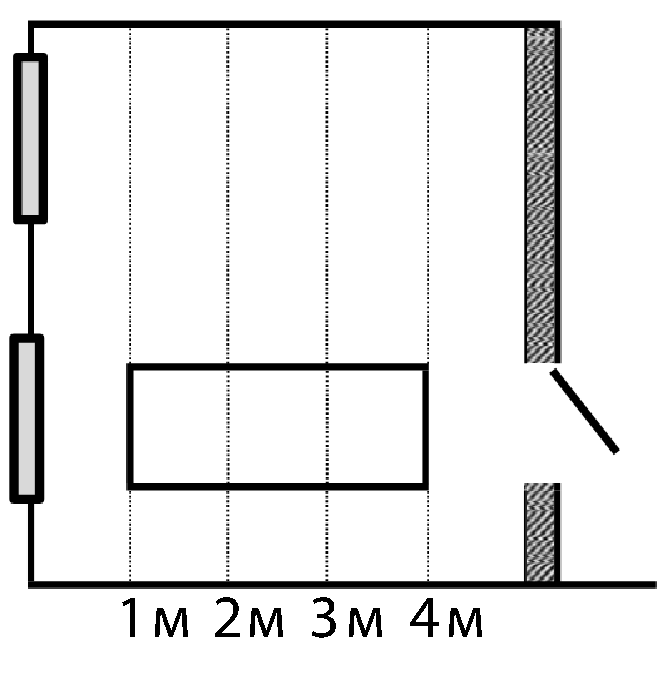
\includegraphics[width=0.2\linewidth]{1.pdf}}
\caption{План приміщення.}
\end{figure}
\end{landscape}

\begin{figure}[h]
\center{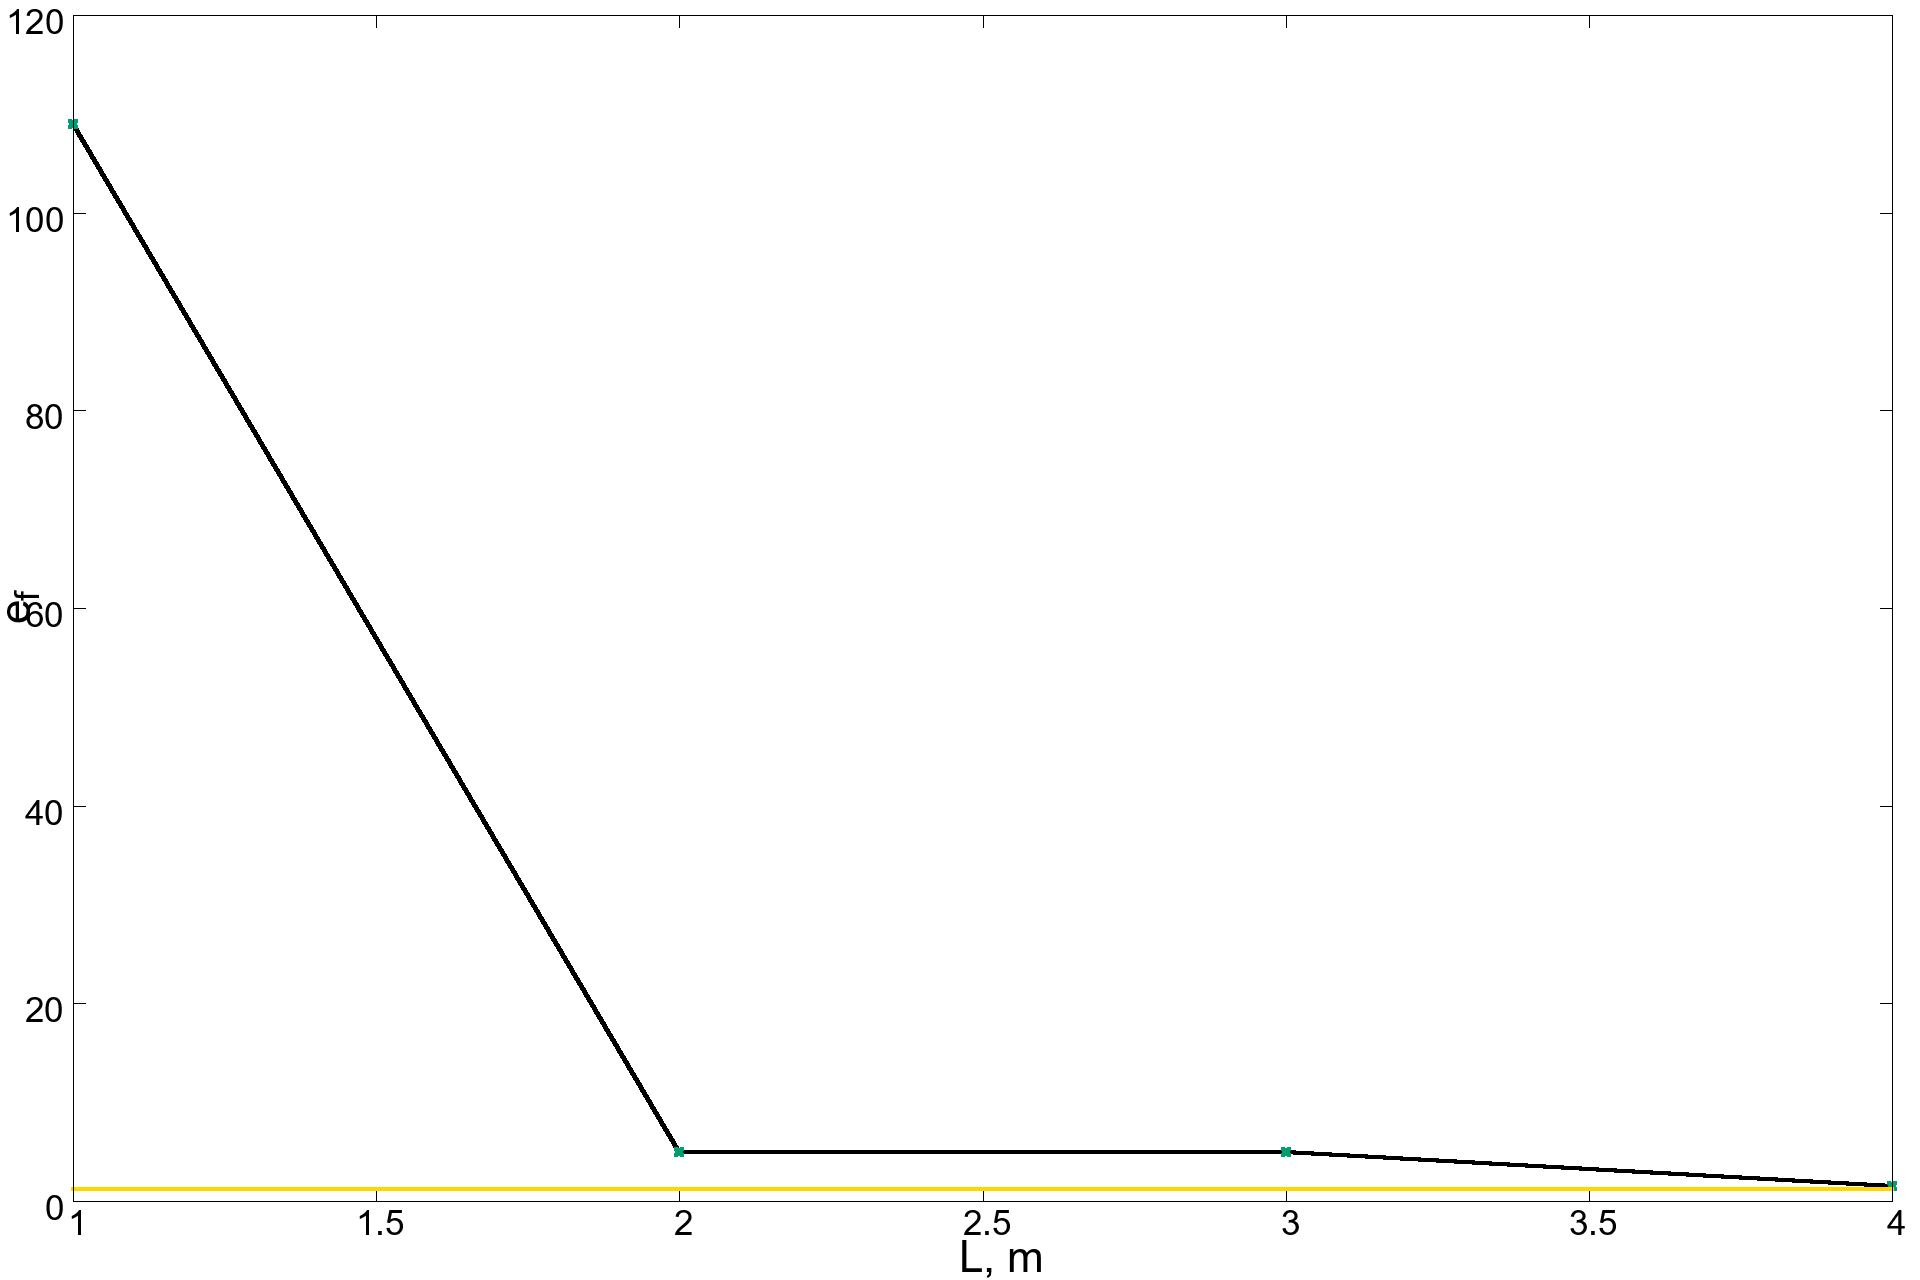
\includegraphics[width=0.9\linewidth]{1.png}}
\caption{Графік залежності фактичного КПО від відстані до вікна L та лінія нормованого КПО.}
\end{figure}
\textbf{Висновок}: за даних умов приміщення відповідаає нормам освітлення, тому потреби у штучному освітленні немає.

















\end{document}
